
\subsection{地表水额度分配与水需求的不匹配}

\begin{figure}[htb]
    \centering
    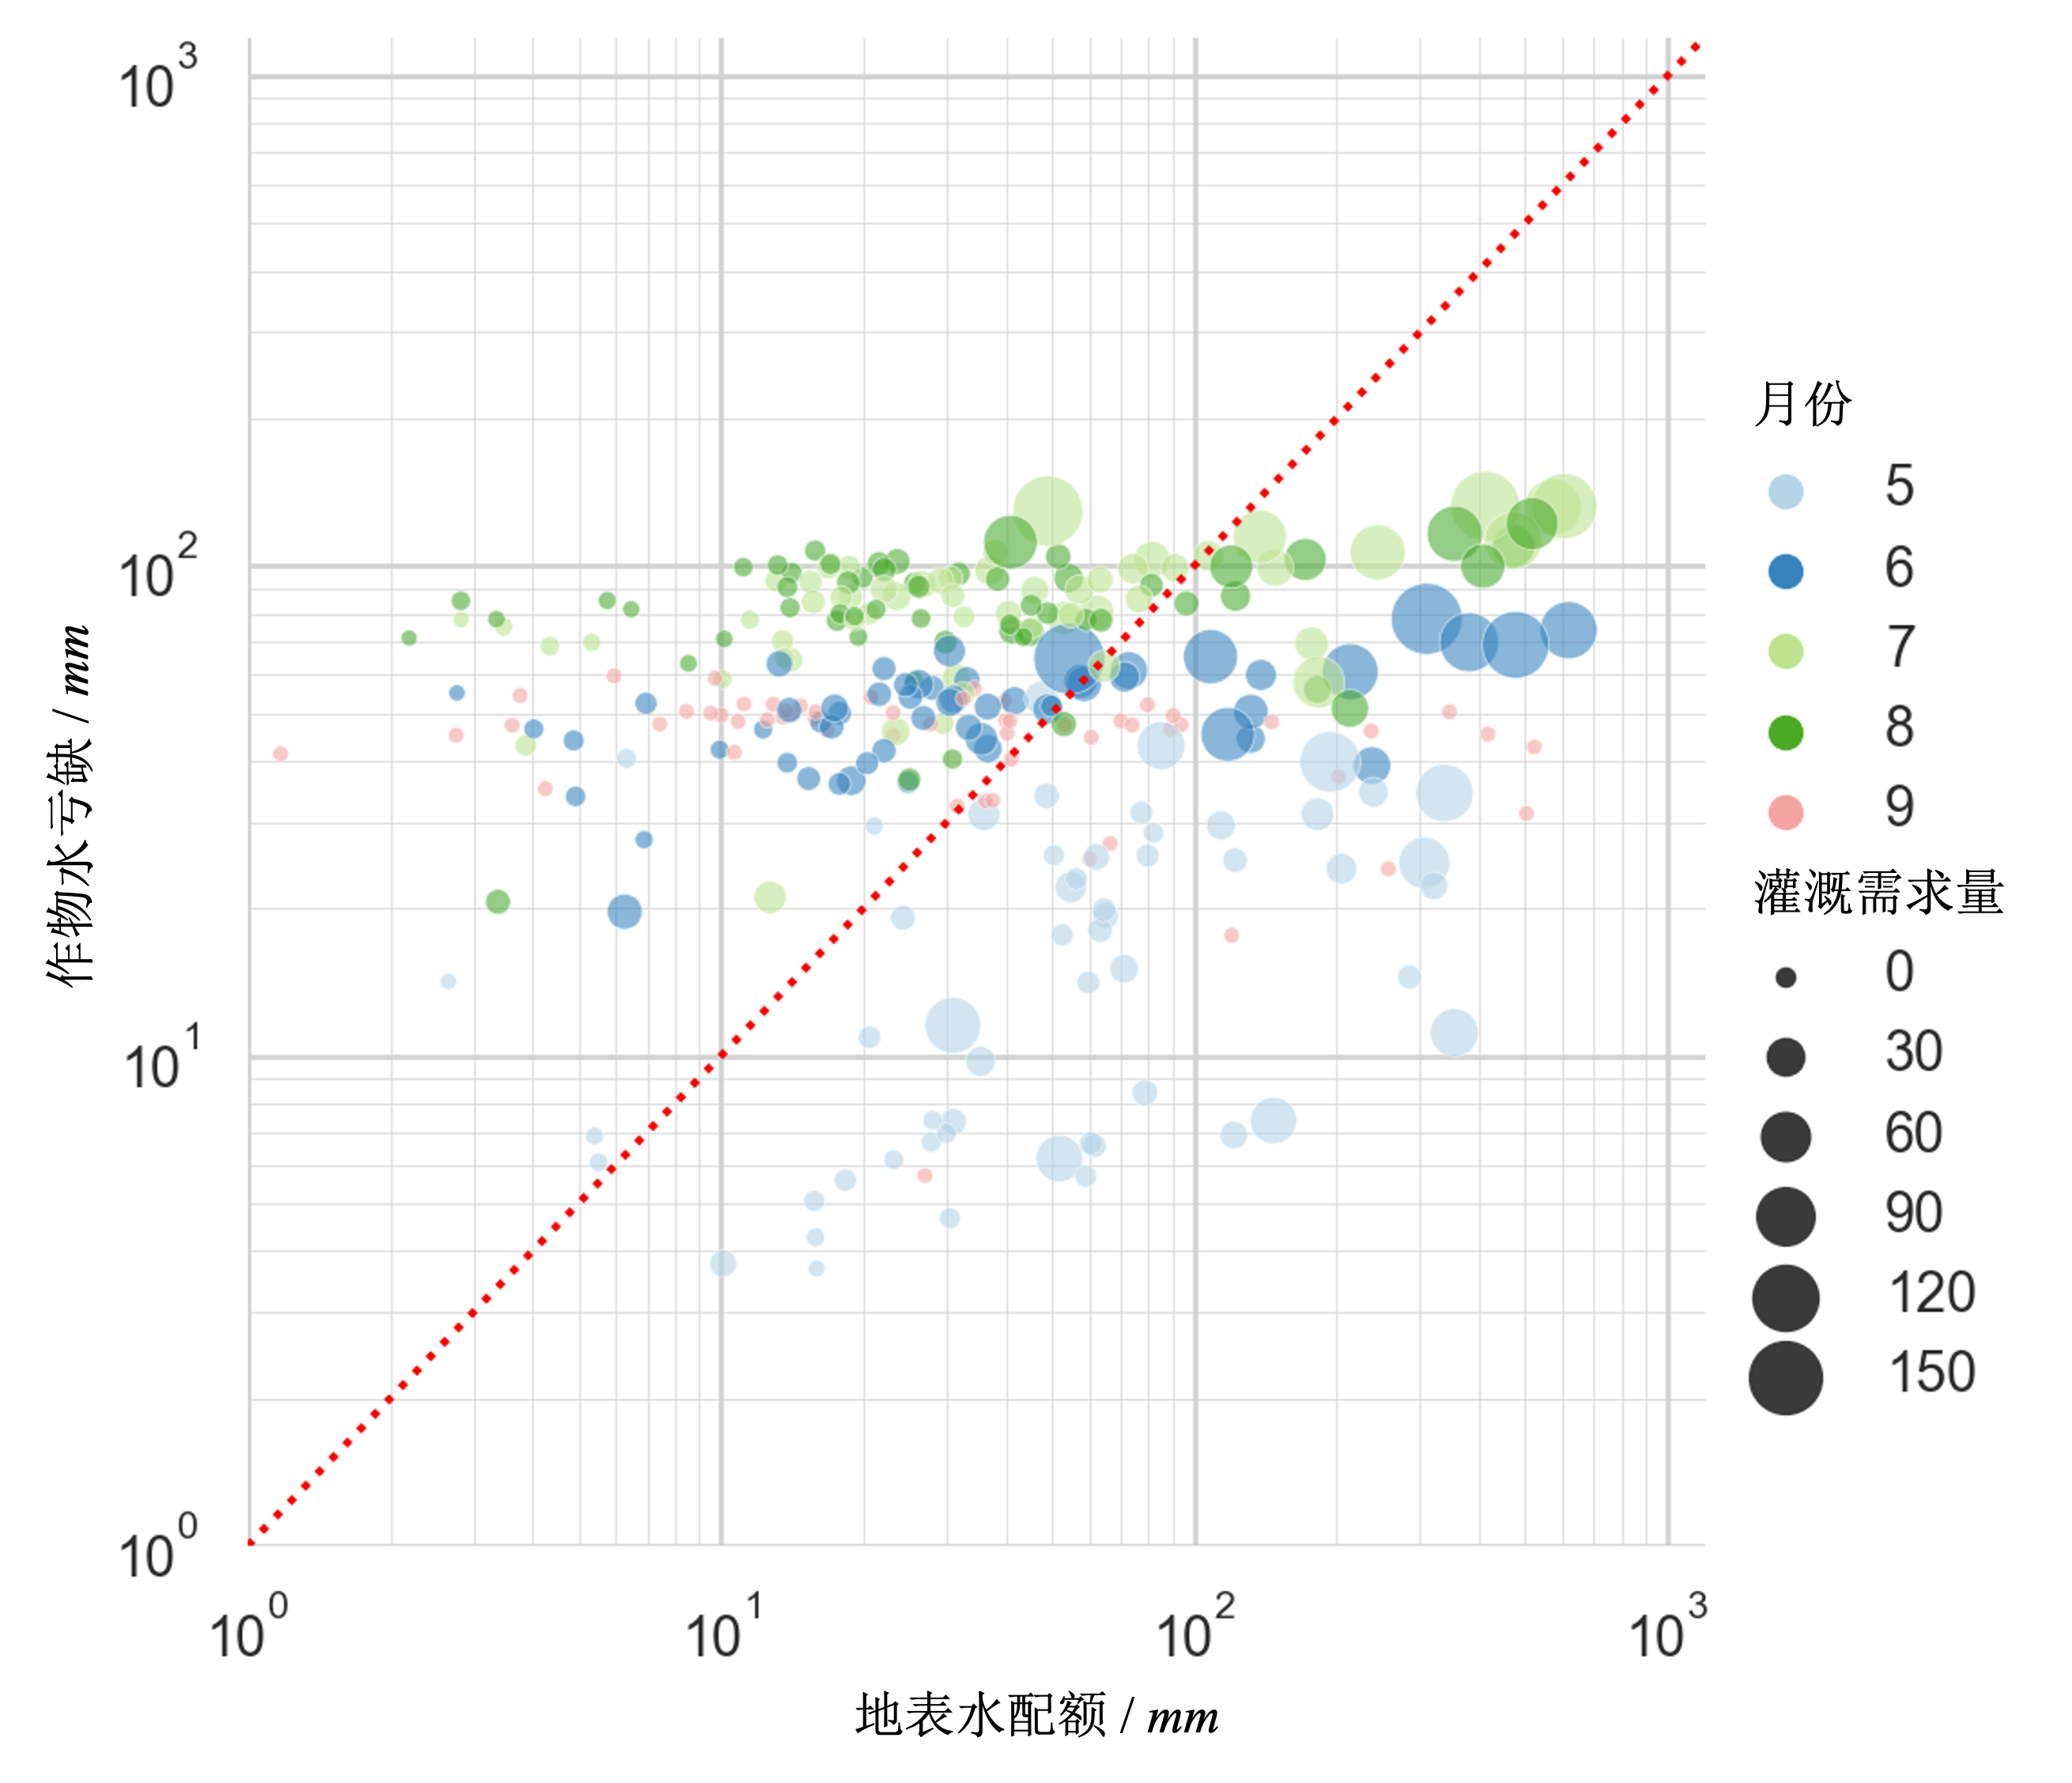
\includegraphics[width=\textwidth]{img/ch6/ch6_matches.png}
    \caption{各地级市月用水额度与用水需求的匹配情况}\label{ch6:fig:matches}
\end{figure}

在图\ref{ch6:fig:matches}中,展示了月尺度水资源配额与作物水资源亏缺的关系。红色虚线表示两者的$1:1$线,右侧表示配额大于作物需求,左侧则表示配额小于作物的绝对用水需求。研究发现,黄河地表水配额与水亏缺存在明显的时空分布不匹配现象。如果供给和需求匹配得很好,大多数气泡点应该落在$1:1$线上。然而实际情况是,气泡的大小代表了统计数据中的地区实际总灌溉用水量,可见水需求量较大的大型灌区也获得了较多的用水配额,容易出现配额供给大于实际作物需求的情况,而在规模偏小的地区则存在水配额供小于求的情况。

此外,气泡的颜色代表了作物生长季的不同月份,发现6月到9月之间的水资源供需失配情况分布比较相似,都是高需水地区有富余,低需水地区存在不足;仅在作物生长的初期(5月)的配额普遍出现水资源配额富余的情况。这些结果表明,在黄河流域,水资源的配额分配存在一定的问题,需要进一步深入研究并制定相应的政策和措施,以保障不同地区的作物水资源供应。

进一步将两者差值映射到空间上,如图\ref{ch6:fig:deficits_maps}所示,可以发现五月的配额大多数地区属于供需平衡的状态,而七、八月的供需匹配情况更为严重,作物需求和配额供给之间的差异部分地区有超过$500mm$的配额富余,但其它地区平均有$100mm$的配额缺口。
在各个月份中,配额富余主要分布在宁夏和内蒙古的河套灌区,这在六月尤其明显;而下游山东灌区则在除五月之外的生长季均有严重的配额不足情况。

\begin{figure}[htb]
    \centering
    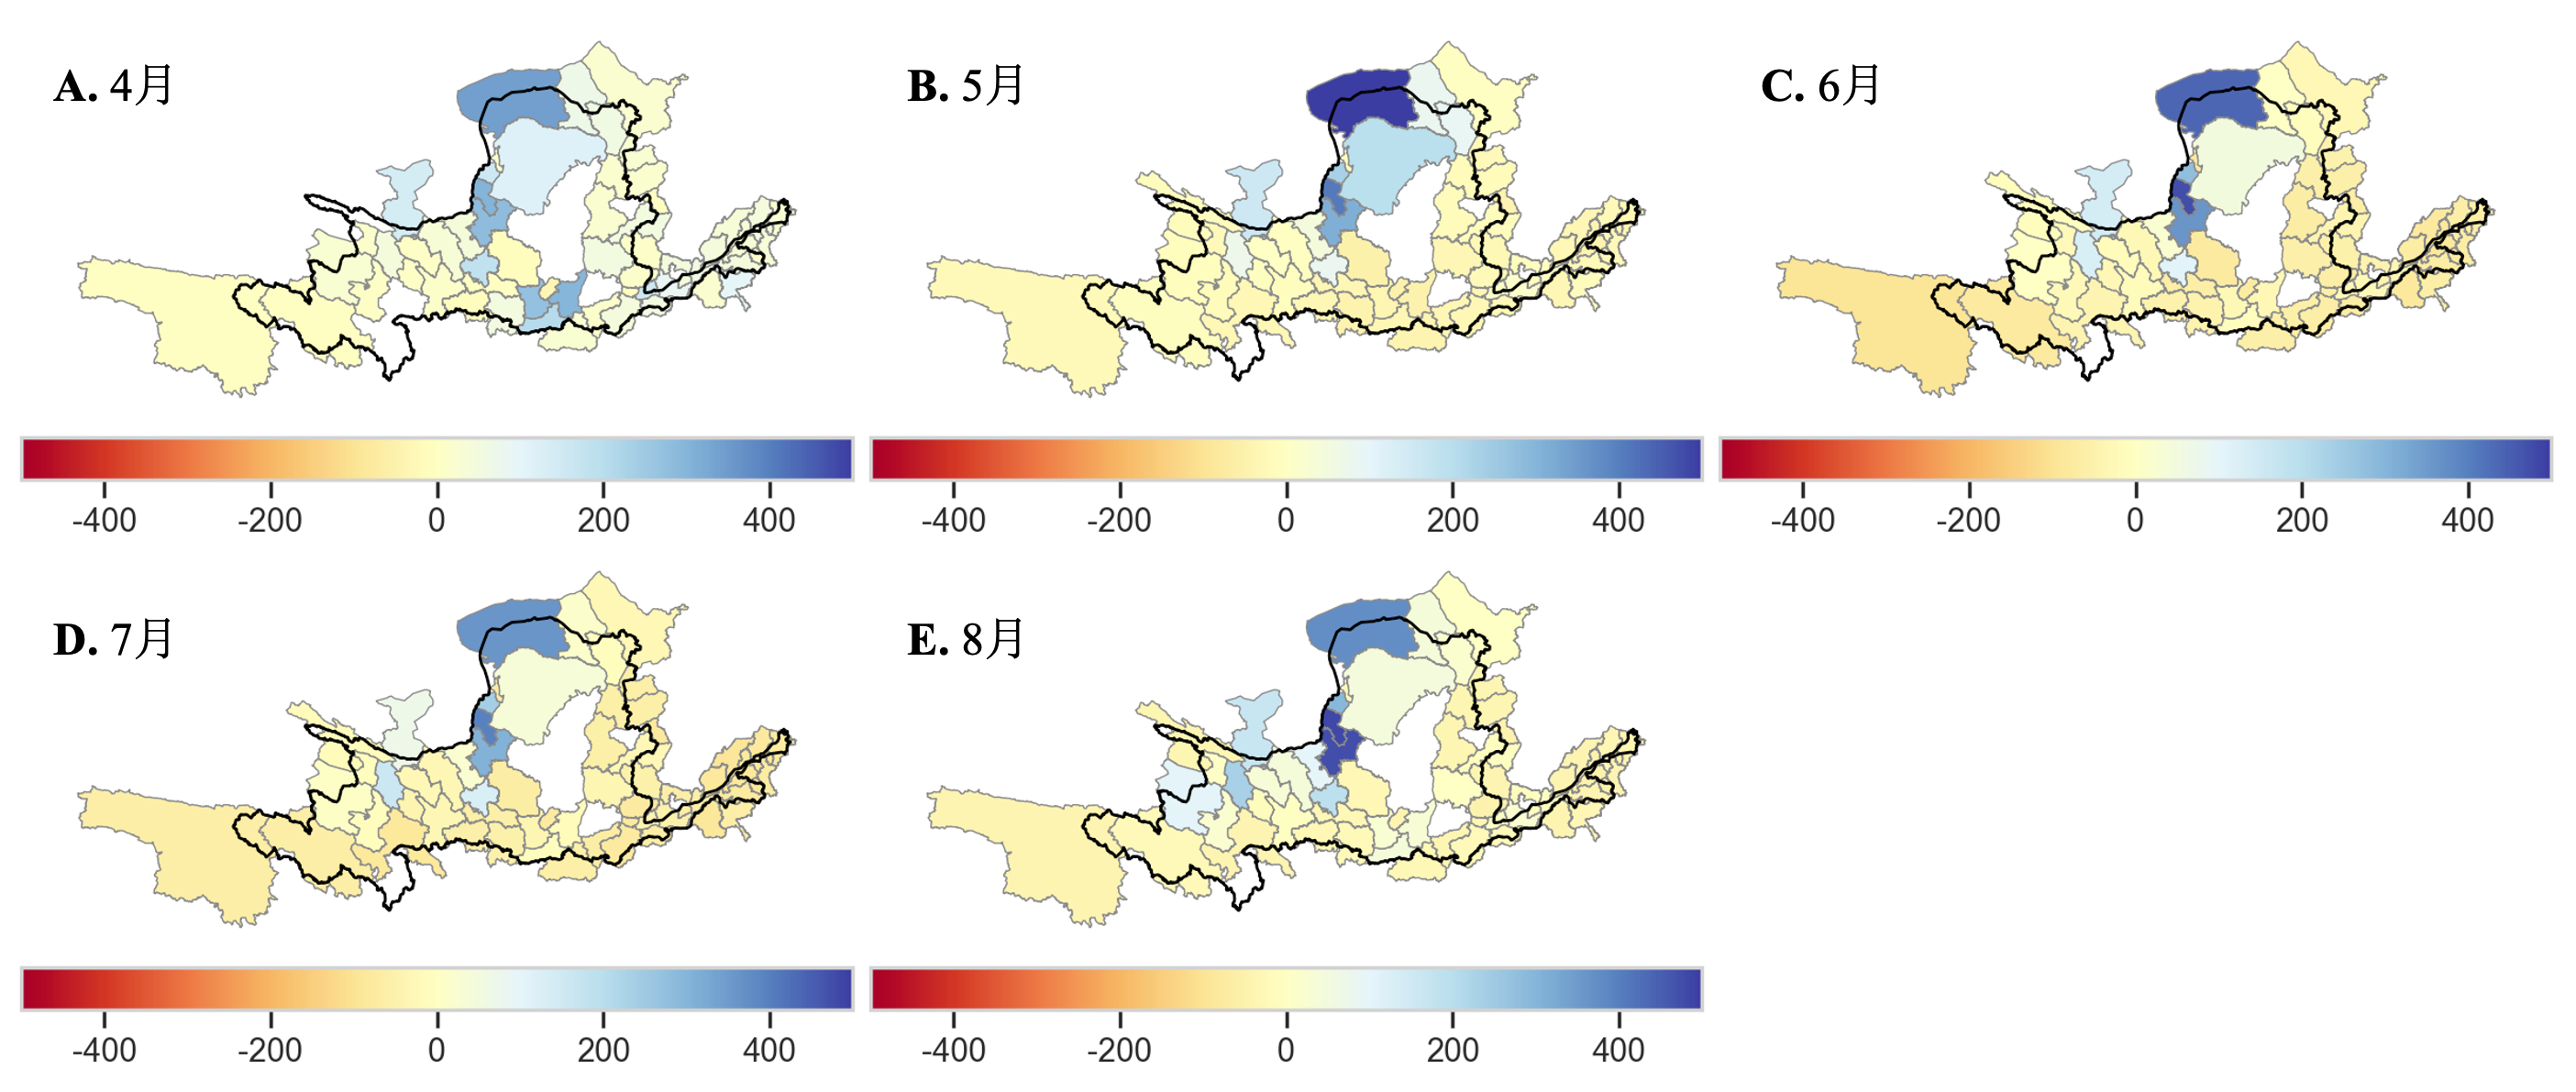
\includegraphics[width=\textwidth]{img/ch6/ch6_deficits_map.png}
    \caption{主要粮食作物生长季黄河地表水配额与作物需水量之差}\label{ch6:fig:deficits_maps}
\end{figure}

\subsection{用水者决策对分水制度变化的响应}

由于社会系统存在决策行为的学习传播过程,违背制度进行超额取水的主体比例会随模拟时间而变化,且随社会模块参数的取值范围存在阈值效应。

配额如果不能满足大多数主体需求,违背制度的决策就会胜出,如青海、内蒙、河南、山东都偏向于违背分水配额,这与第五章识别的超额取水模式大体一致。

\begin{figure}[htb]
    \centering
    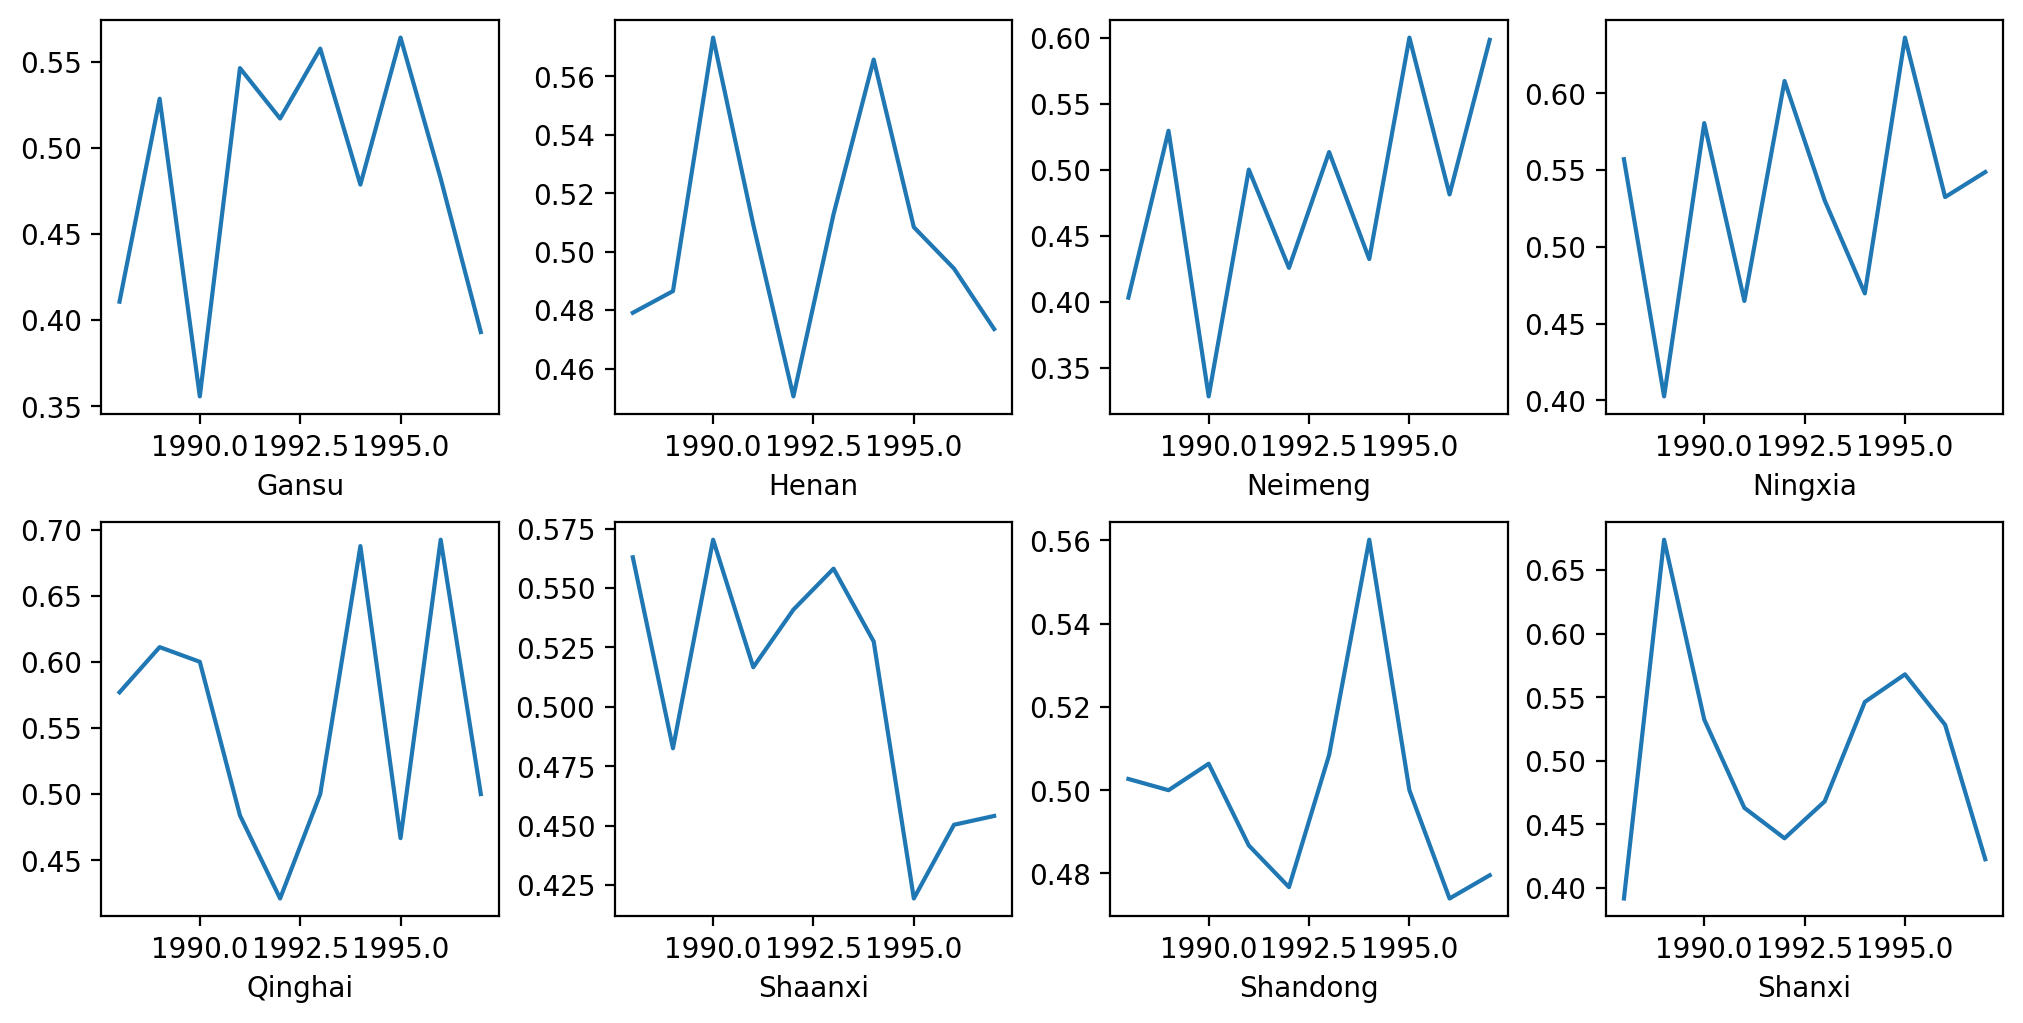
\includegraphics[width=\textwidth]{img/ch6/ch6_threshold.png}
    \caption{改变配额制度}\label{fig:xfig0}
\end{figure}

\subsection{用水来源对分水制度变化对的响应}

模型能够模拟各省份绿水(降水+土壤水)/蓝水(地表/地下水)的使用情况
黄河流域作物生长的主要水源是绿水。研究表明,各省在总体上保持了蓝水使用占比持续下降的趋势,但是对用蓝/绿水比例的影响并不明显,仅有个别省份存在突变。
因此,为了更好地保护黄河流域的水资源,需要对各省的蓝水和绿水的使用情况进行深入研究,以便更好地理解不同省份之间的差异和变化。
此外,还需要进一步探讨各省份之间绿水资源的分配情况,以及如何更好地利用绿水资源来支持作物的生长和发展。这些研究结果对于制定更好的水资源管理政策和措施具有重要的意义。

\begin{figure}[htb]
    \centering
    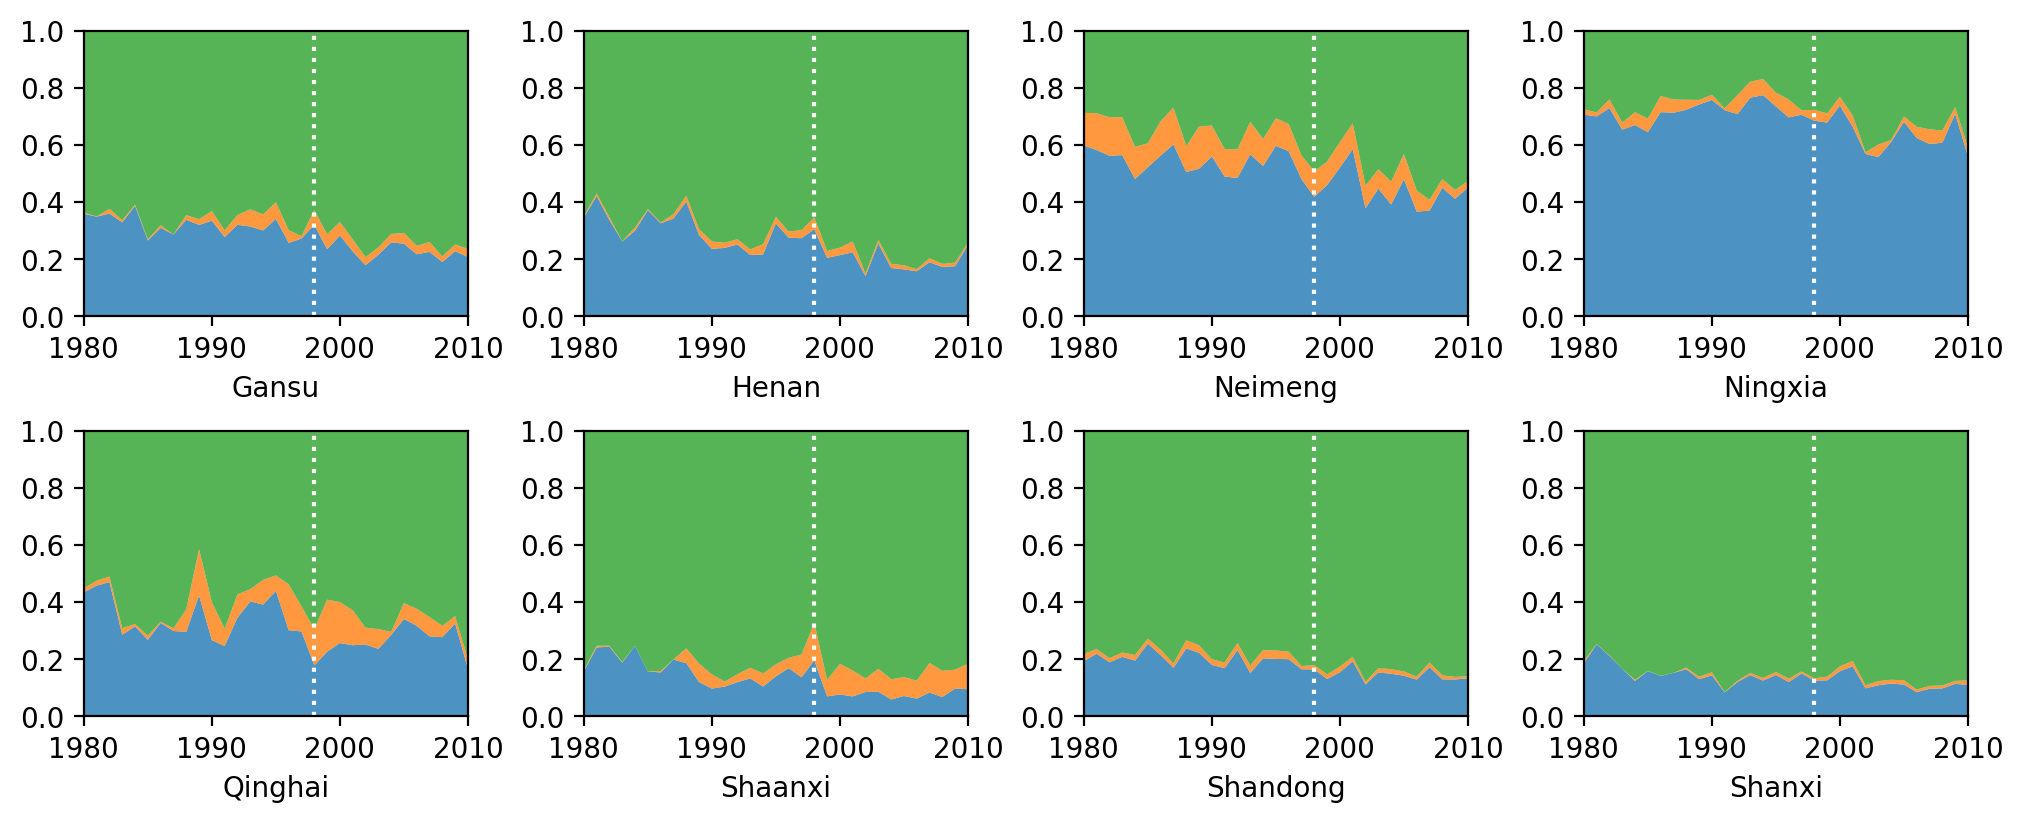
\includegraphics[width=\textwidth]{img/ch6/ch6_green_blue_water.png}
    \caption{黄河流域主要农作物用水来源的比例变化}\label{ch6:fig:sources}
\end{figure}

\subsection{地下水开采对分水制度变化的响应}

地下水使用量是分析黄河流域分水制度变化影响的重要指标。研究表明,分水制度变化对黄河流域的地下水使用量带来的影响较为明显。
具体来说,中游地区持续增加地下水的开采量,而下游地区在1987年分水制度提出之初期就开始推动节水改革。
而上游地区则先加大了地下水的开采量,在1998年统一调度制度实施后才大力推行节水改革。这些不同的反应与各地的经济发展和地下水资源的分布有关。
因此,在制定水资源管理政策和措施时,需要充分考虑不同地区的特点和实际情况,并针对性地制定相应的政策和措施。
同时,需要进一步深入研究分水制度变化对地下水使用量的影响机制,为制定更有效的水资源管理政策提供科学依据。

\begin{figure}[htb]
    \centering
    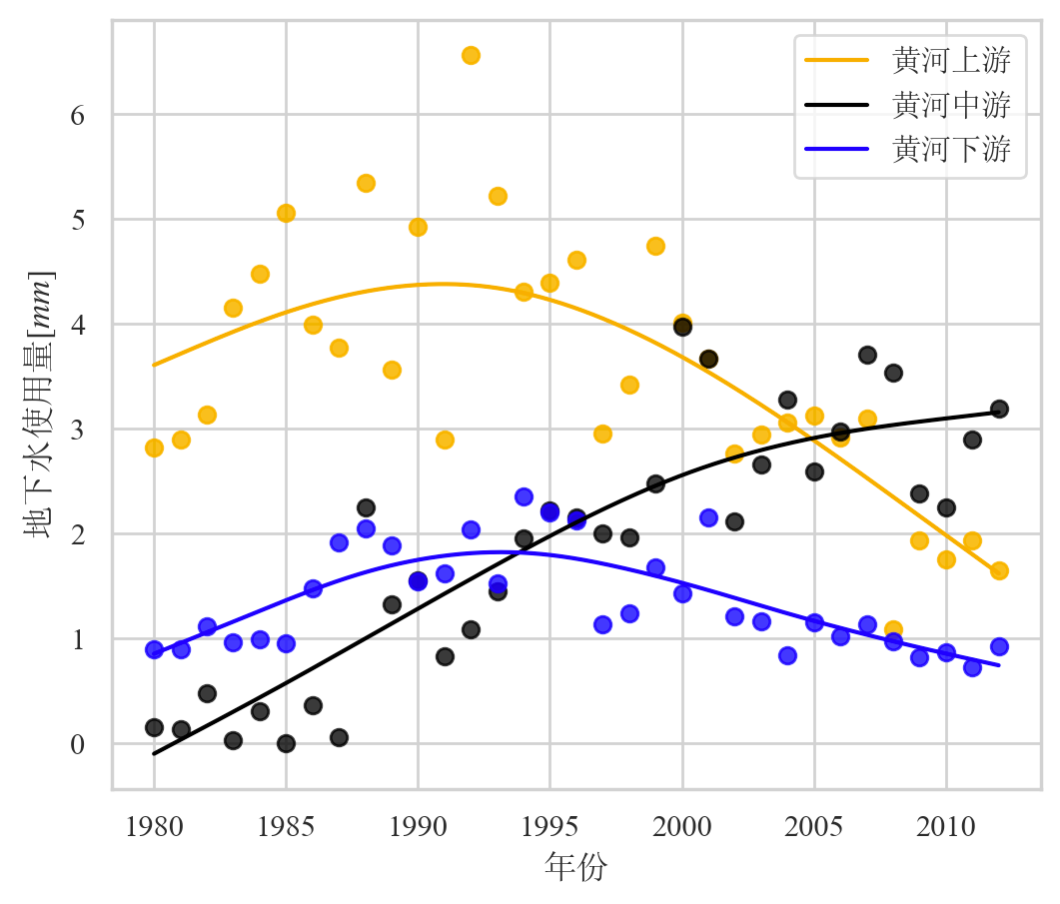
\includegraphics[width=0.6\textwidth]{img/ch6/ch6_groundwater.png}
    \caption{黄河流域、中、下游地下水开采量对分水制度变化的响应}\label{ch6:fig:groundwater}
\end{figure}